\documentclass[12pt,a4paper]{article}
\usepackage[english, science, large]{../template/ku-frontpage}
\usepackage{tabularx}
\usepackage{ltablex}
\hypersetup{
    colorlinks=false,
    pdfborder={0 0 0},
}
\begin{document}

\title{ACS Theory Assignment 1}
\subtitle{}

\author{Kai Arne S. Myklebust, Silvan Adrian}
\date{Handed in: \today}
	
\maketitle
\tableofcontents

\section{Question 1: Techniques for Performance}
\subsection{Question 1.1}
Concurrency may improve latency, but one must be careful because of locking and correctness. While using concurrency two processes may need to write on the same element and then one process needs to be locked and latency may get worse.
\subsection{Question 1.2}
\textbf{Batching} is when you run multiple requests at once. One example is billing in a credit card company, where they run a monthly billing cycle. All data gets collected at the end of the month and sent at once. \\
\textbf{Dallying} is when you wait until you have some requests accumulated and then run them. One example is where a request comes in too overwrite a disk block, but waits for more requests that may overwrite the same disk block. Then the first request would not be needed anymore. \\
Batching may improve latency and throughput, but dallying typically incurs a latency penalty because it waits for more requests.
\subsection{Question 1.3}
Yes, because it makes one optimized path for common requests, where it tries to eliminate the need for reads and writes in lower level memory. But only goes deeper when needed.

\section{Question 2: Fundamental Abstractions}
\subsection{Question 2.1}


\subsection{Question 2.2}

\subsection{Question 2.3}

\subsection{Question 2.4}

\section{Question 3: Serializability \& Locking}

\subsection{Precedence graph}
\subsubsection{Schedule 1}
Yes it is conflict-serializable, because there is no cycle in the precedence graph.
\begin{figure}[!htb]
	\center
	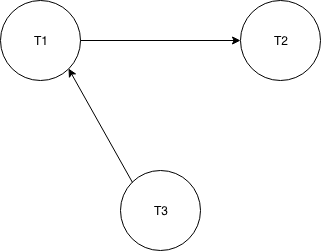
\includegraphics[width=0.5\textwidth]{img/schedule1}
	\caption{Precedence graph of schedule 1}
\end{figure}\\
\subsubsection{Schedule 2}
Yes, since the precedence graph has no precedences and therefore also no cycle.

\subsection{Strict 2PL scheduler}

\subsubsection{Schedule 1}
Transaction 2 has a write on X but there is already a shared lock on X in T1, that's why it has to abort.
\begin{figure}[!htb]
	\center
	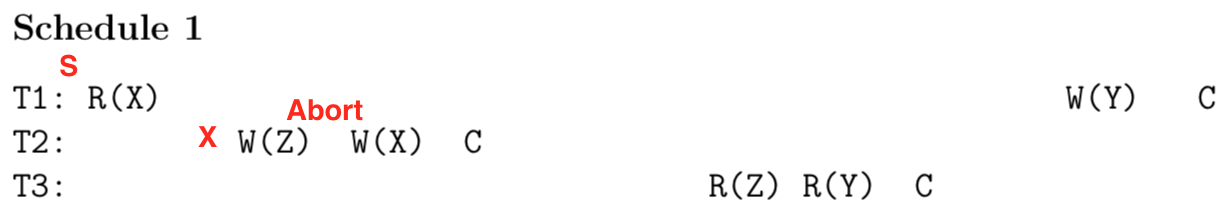
\includegraphics[width=\textwidth]{img/Schedule1_strict2PL}
	\caption{Schedule 1, strict 2PL}
\end{figure}


\subsubsection{Schedule 2}
Yes it can be generated by strict 2PL scheduler, see figure.
\begin{figure}[!htb]
	\center
	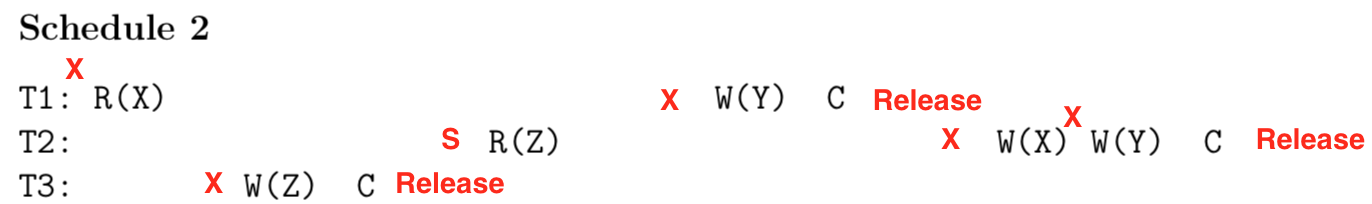
\includegraphics[width=\textwidth]{img/Schedule2_strict2PL}
	\caption{Schedule 2, strict 2PL}
\end{figure}

\section{Question 4: Optimistic Concurrency Control}

\end{document}}